\clearpage
\section{Supplementary material}
\label{sec:Supplementary}

\begin{figure}[h!]
\centering
%%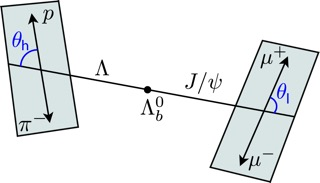
\includegraphics[width=0.65\textwidth]{images_and_tables/Angular/angles.pdf}
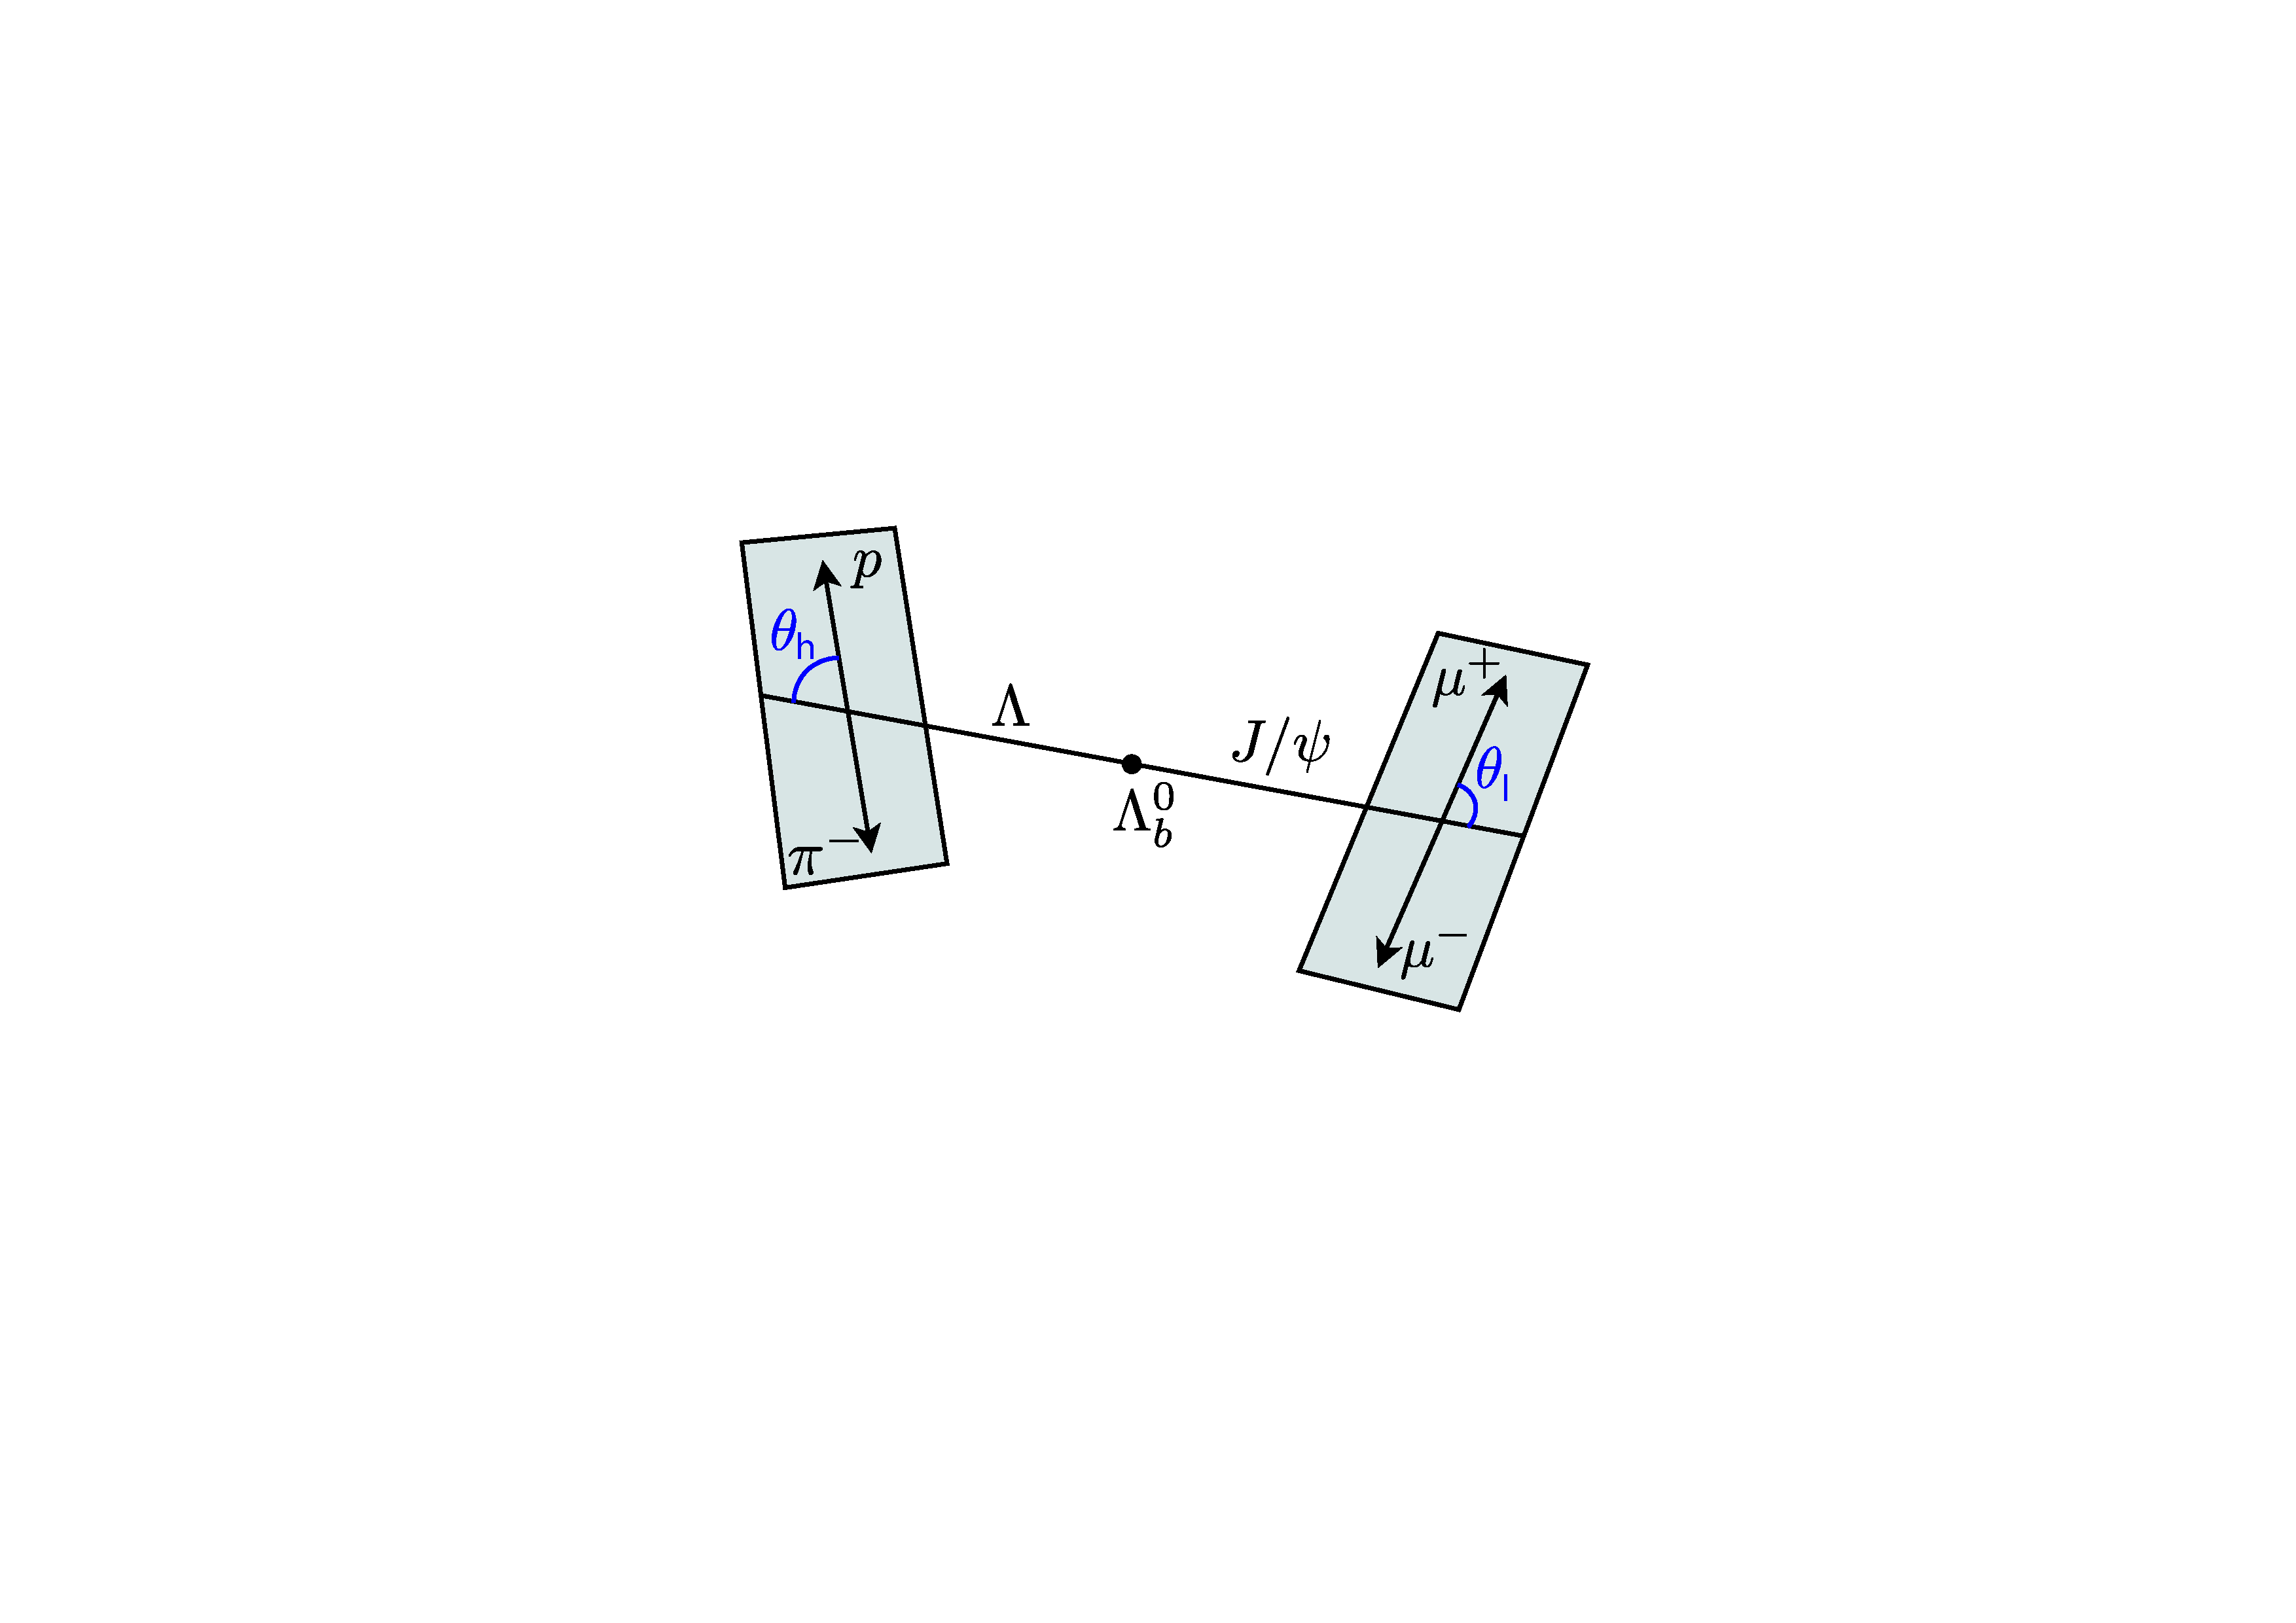
\includegraphics[width=0.65\textwidth]{figure11.pdf}
\caption{Graphical representation of the angles for the \decay{\Lb}{\Lz\mumu} decay.}
\end{figure}

\begin{figure}[h!]
\centering
%%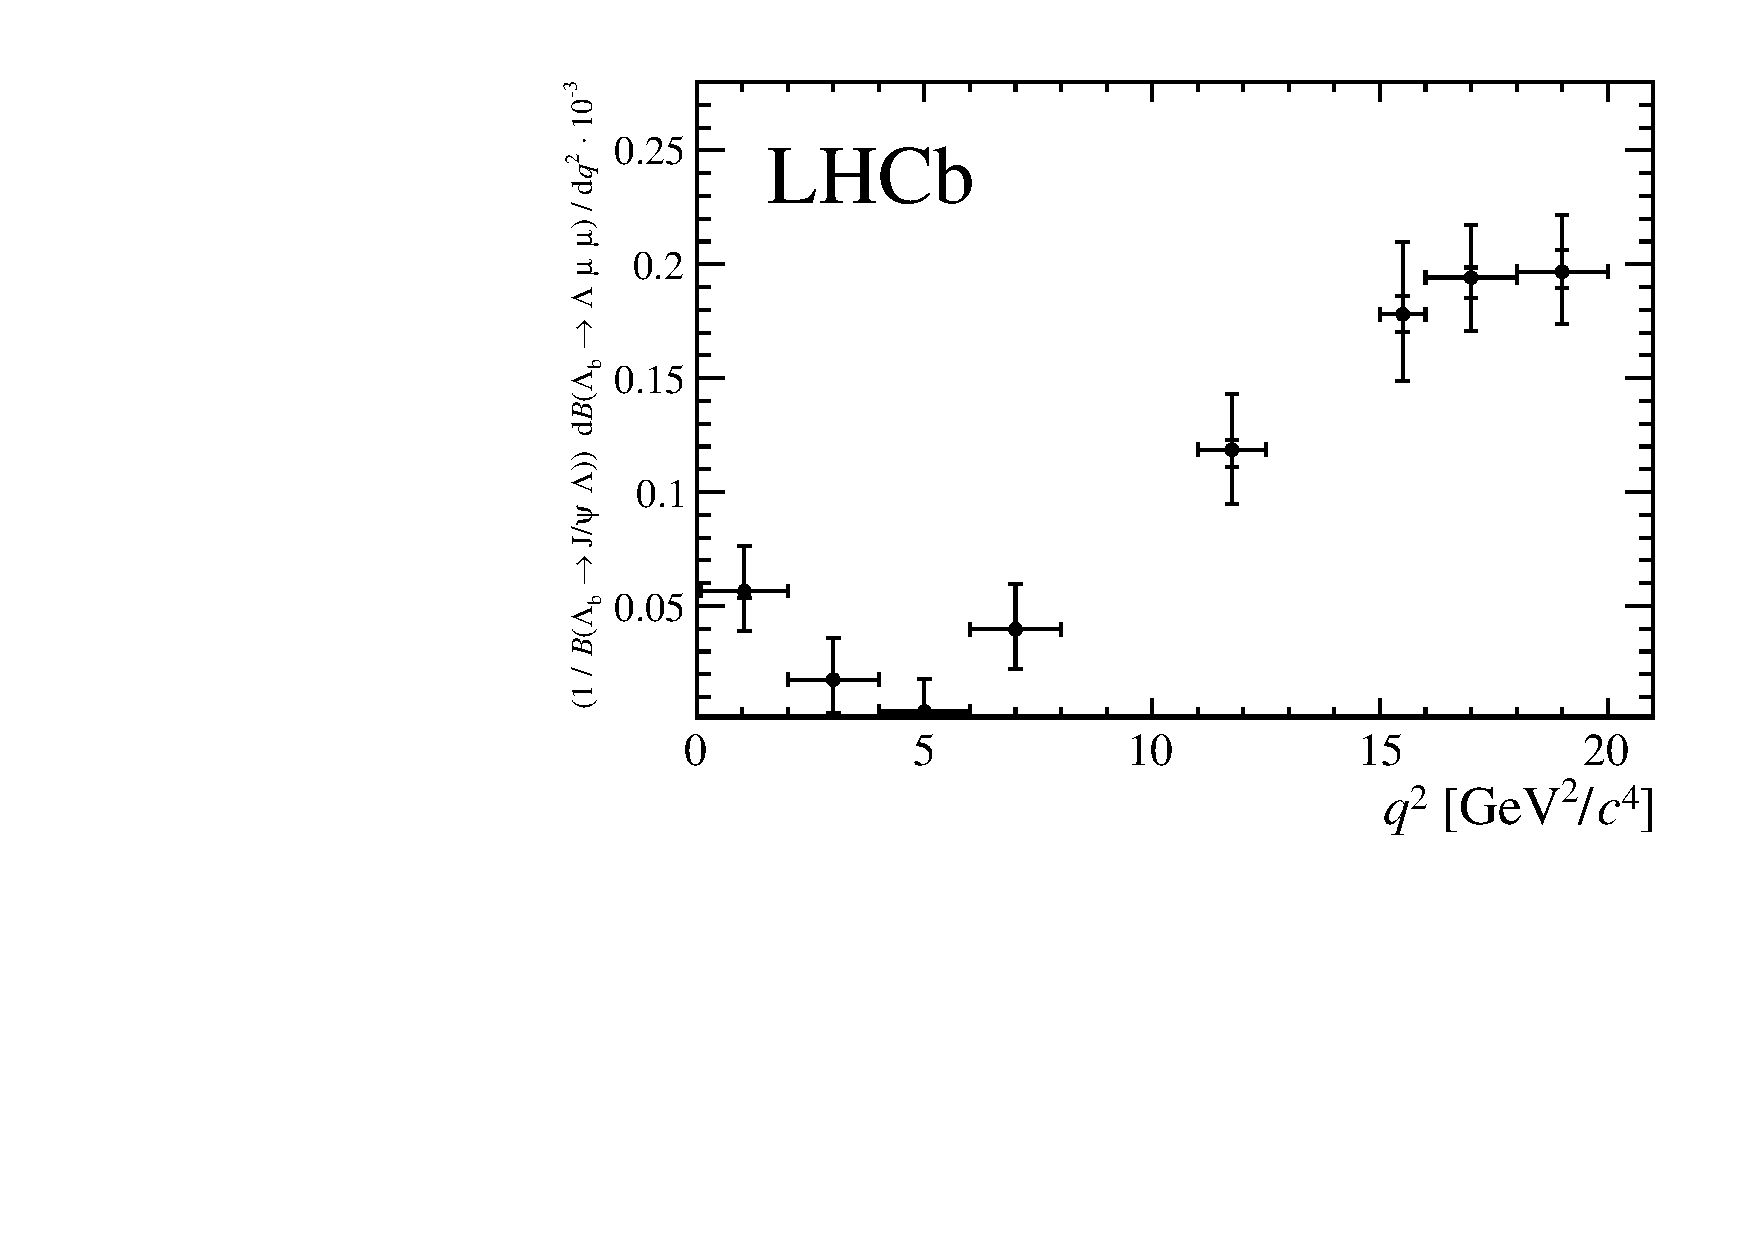
\includegraphics[width=0.65\textwidth]{images_and_tables/BR/combined_result_2err.pdf}
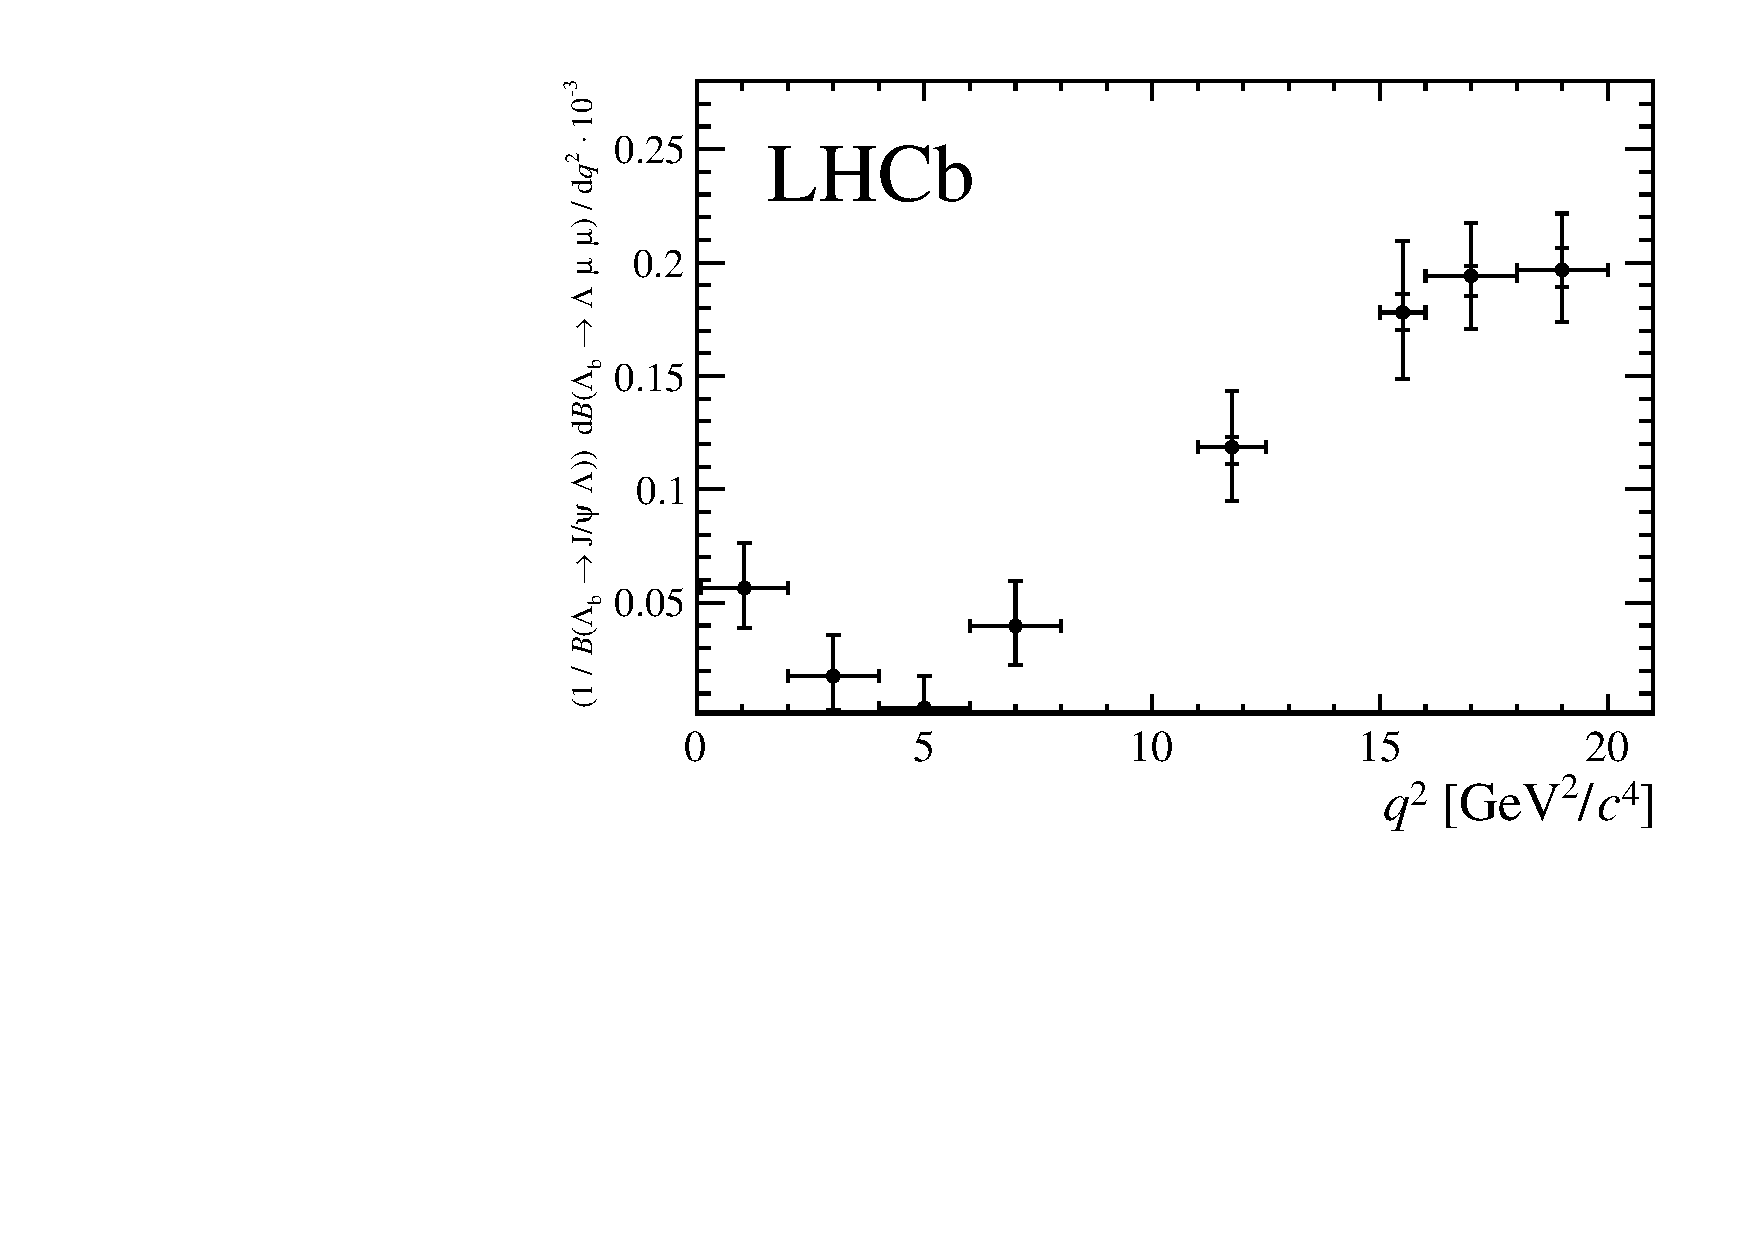
\includegraphics[width=0.65\textwidth]{figure12.pdf}
\caption{Branching fraction of the \decay{\Lb}{\Lz\mumu} decay
  normalised to the \decay{\Lb}{\jpsi\Lz} mode. The inner error
  represents the systematic error and the outer error the total
  error.} 
\label{fig:RelBR}
\end{figure}

\begin{figure}[tbp]
%%\centering \includegraphics[width=0.65\textwidth]{images_and_tables/BR/fit_All_lowQ2.pdf}
\centering 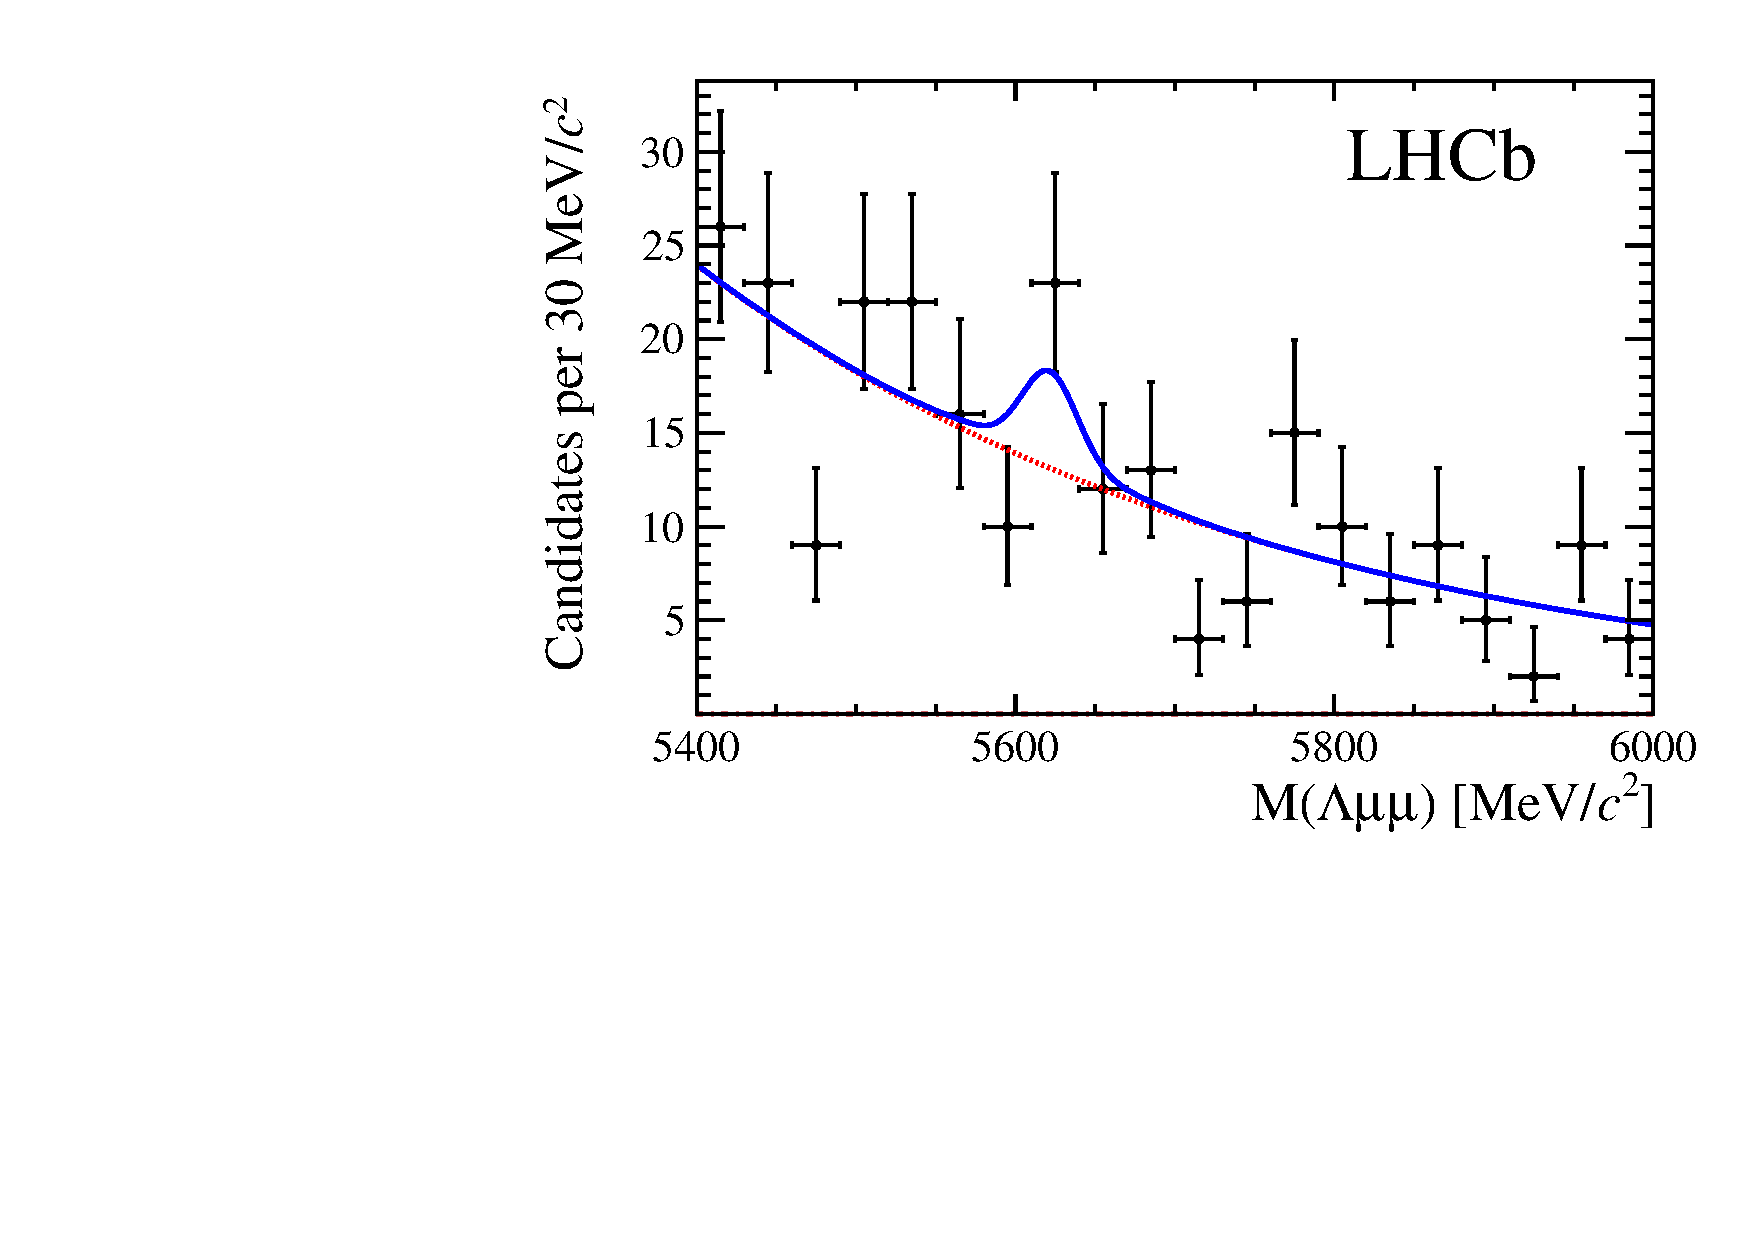
\includegraphics[width=0.65\textwidth]{figure13.pdf}
\caption{\small Invariant mass distribution of the
  \decay{\Lb}{\Lz\mumu} candidates, integrated over the region  $1.1 < \qsq < 6.0$ \gevgevcccc 
  together with the fit function described in the text.  The points show data,
  the solid (blue) line is the overall fit function and the dotted (red) line the
  combinatorial background.}
\label{fig:totalFitRare_lowq2}
\end{figure}

\begin{figure}[hbtp]
\centering
%%\includegraphics[width=0.8\textwidth]{images_and_tables/Angular/fL.pdf}
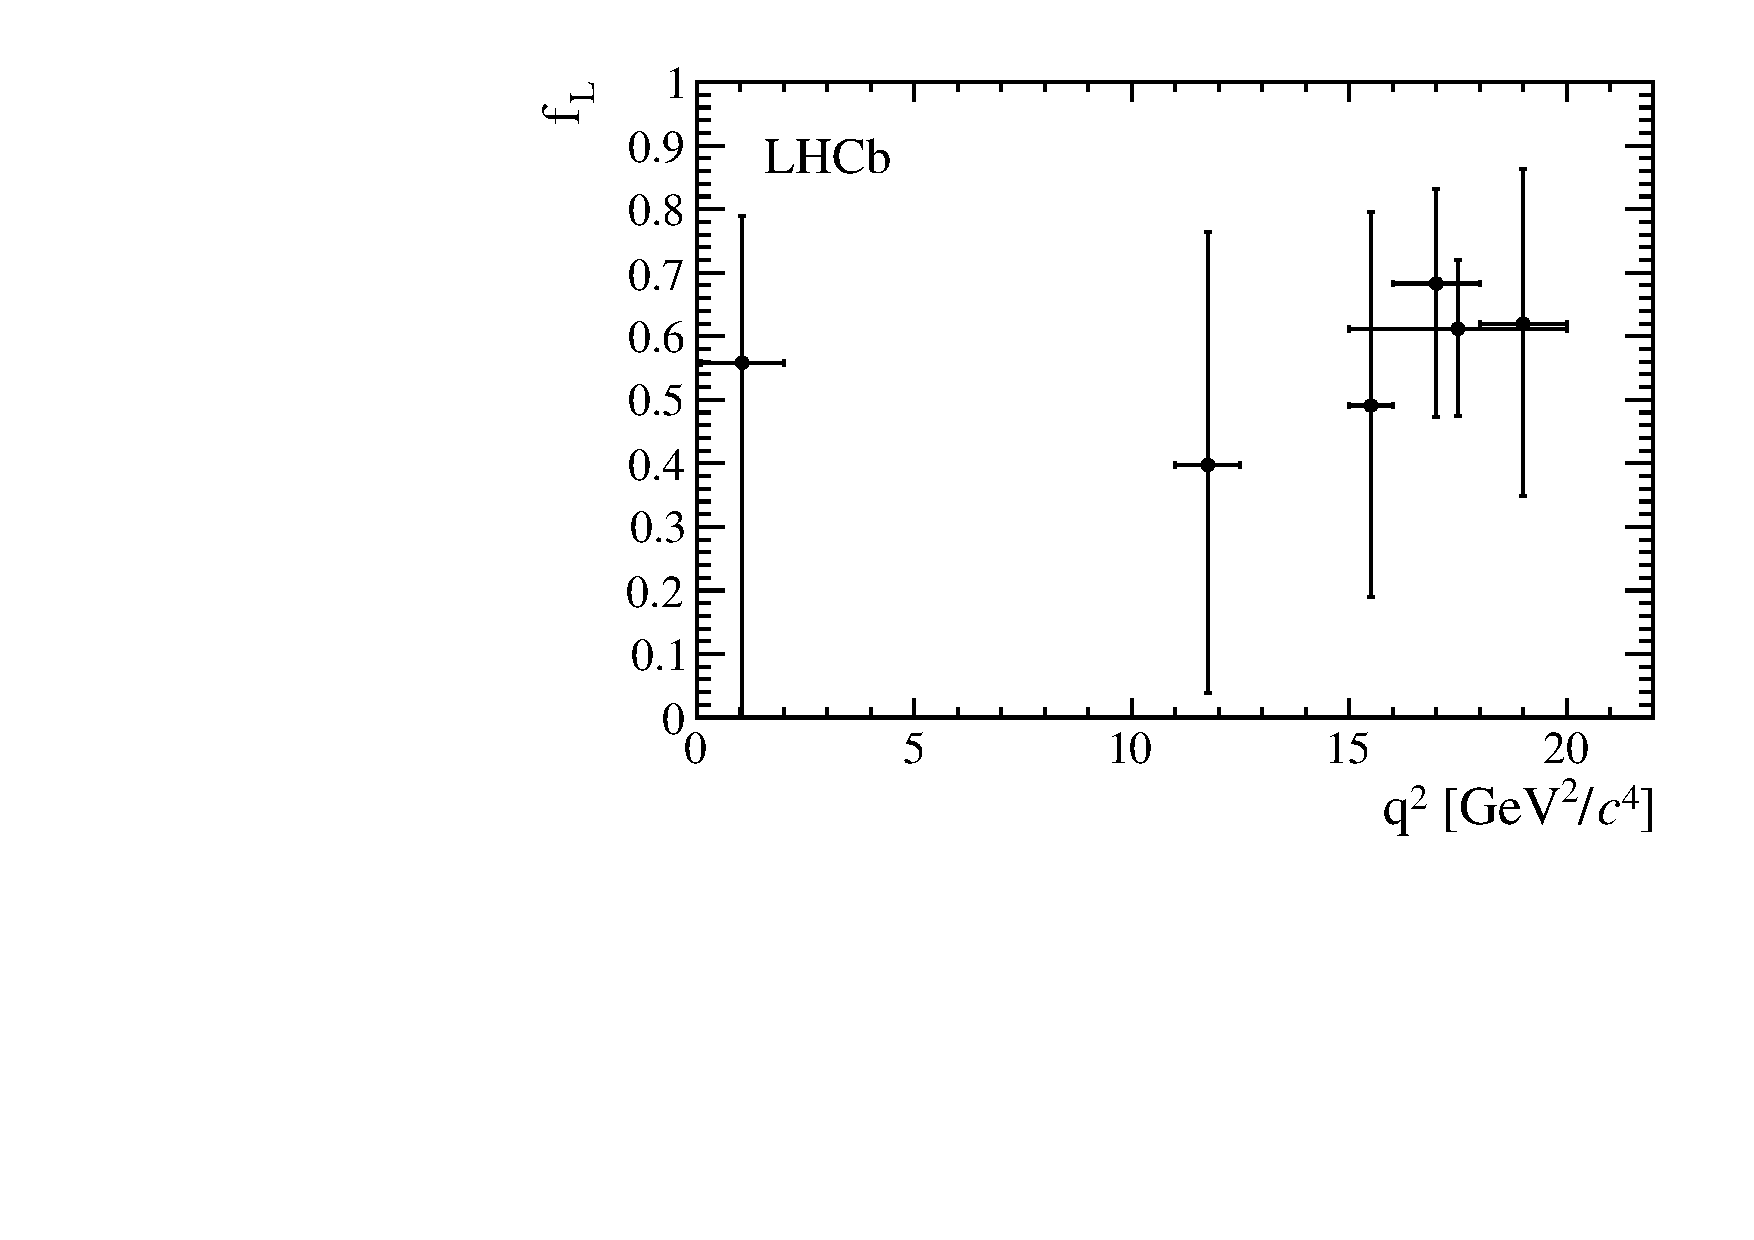
\includegraphics[width=0.8\textwidth]{figure14.pdf}
\caption{The measured fraction of longitudinally polarised dimuons,
  $f_{\rm L}$.}
\label{fig:fL}
\end{figure}

\clearpage
